\documentclass[a5paper,12pt]{article}
\usepackage{../../style}


\newcommand{\montitre}{Algorithmique }


\begin{document}

\fiche{Définitions}
\titre{Modèle} : Une représentation du monde réel. En physique et en maths, il prend ses valeurs dans des espaces denses, en informatique dans des espaces discrets finis.\\

\titre{Problème/Algorithme/Programme} Ne pas confondre les 3 notions.\\

\titre{Problème} : Du grec problema (jeté devant ie obstacle). Un problème est constitué d'une situation initiale et d'un but à atteindre pour la situation finale.

\titre{Algorithme} : (Al Khwarizmi : 820 ap JC) Une façon systématique de procéder pour faire quelque chose en un nombre fini d'étapes élémentaires.\\

\titre{Programme} : Mise en oeuvre concrète d'un algorithme dans un langage de programmation.\\
   
\titre{Preuve de programme} : On peut prouver qu'il y a conformité entre le modèle mathématique et le programme, mais pas qu'il répond à la sémantique naturelle du problème (ie qu'il marche). Il faudrait pour cela être capable de tester TOUS les cas possibles.\\

\titre{Syntaxe/Sémantique} : La syntaxe est maîtrisable, mais pas la sémantique.\\

\titre{Ambiguité} : Les langages naturels sont ambigus ("Rogrigue, as tu du coeur?"), tandis que les langages de programmation ne le sont pas $\impl$ déterminisme.\\

\titre{Compilateur} : \begin{enumerate}
	\item \titre{parsing} ou \titre{analyse lexicale} : Assemble les symboles en groupes formant des expressions. 
	\item \titre{analyse syntaxique} : Vérifie que les expressions sont grammaticalement correctes.
	\item \titre{table des symboles} : Visibilité des symboles, renommage, contrôle de type.
	\item \titre{génération de code} : syntaxe abstraite.
\end{enumerate}

\titre{Abstrait} : En informatique, abstrait signifie : on oublie certaines informations.  

\titre{Grammaire regex} : Fait elle partie des grammaires hors contexte ? (oui ?)

\newpage

\titre{Grammaire hors contexte} : Ne dépend pas du contexte. Elle est constituée de : 
\begin{itemize}
	\item Un ensemble $T$ de symboles terminaux (alphabet des symboles)
	\item Un ensemble $N$ de symboles non-terminaux ($T\cap N =\vide$) (alphabet des variables -> à voir comme une catégorie.
	\item Un ensemble $R$ de règles (couples $(x,y)$ notés $x \rightarrow y$, de mots sur $V\cup N$) 
	\item Un symbole de départ $S\in N$
\end{itemize}

\titre{Exemple} : Un entier 
\begin{itemize}
	\item $T = \{-,0,1,2,3,4,5,6,7,8,9\}$
	\item $N = \{<chiffre>,<entier>,<suite>\}$
	\item Règles : \begin{itemize}
		\item $<entier> ::= (-|\varepsilon) <origine><suite>$ 
		\item $<suite> ::= (0|<chiffre>)<suite> | \varepsilon$
		\item $<chiffre> ::= 1|2|3|4|5|6|7|8|9$
		\end{itemize}
	\item $S = <entier>?$
\end{itemize}
Construction de l'arbre de $243$ :\\
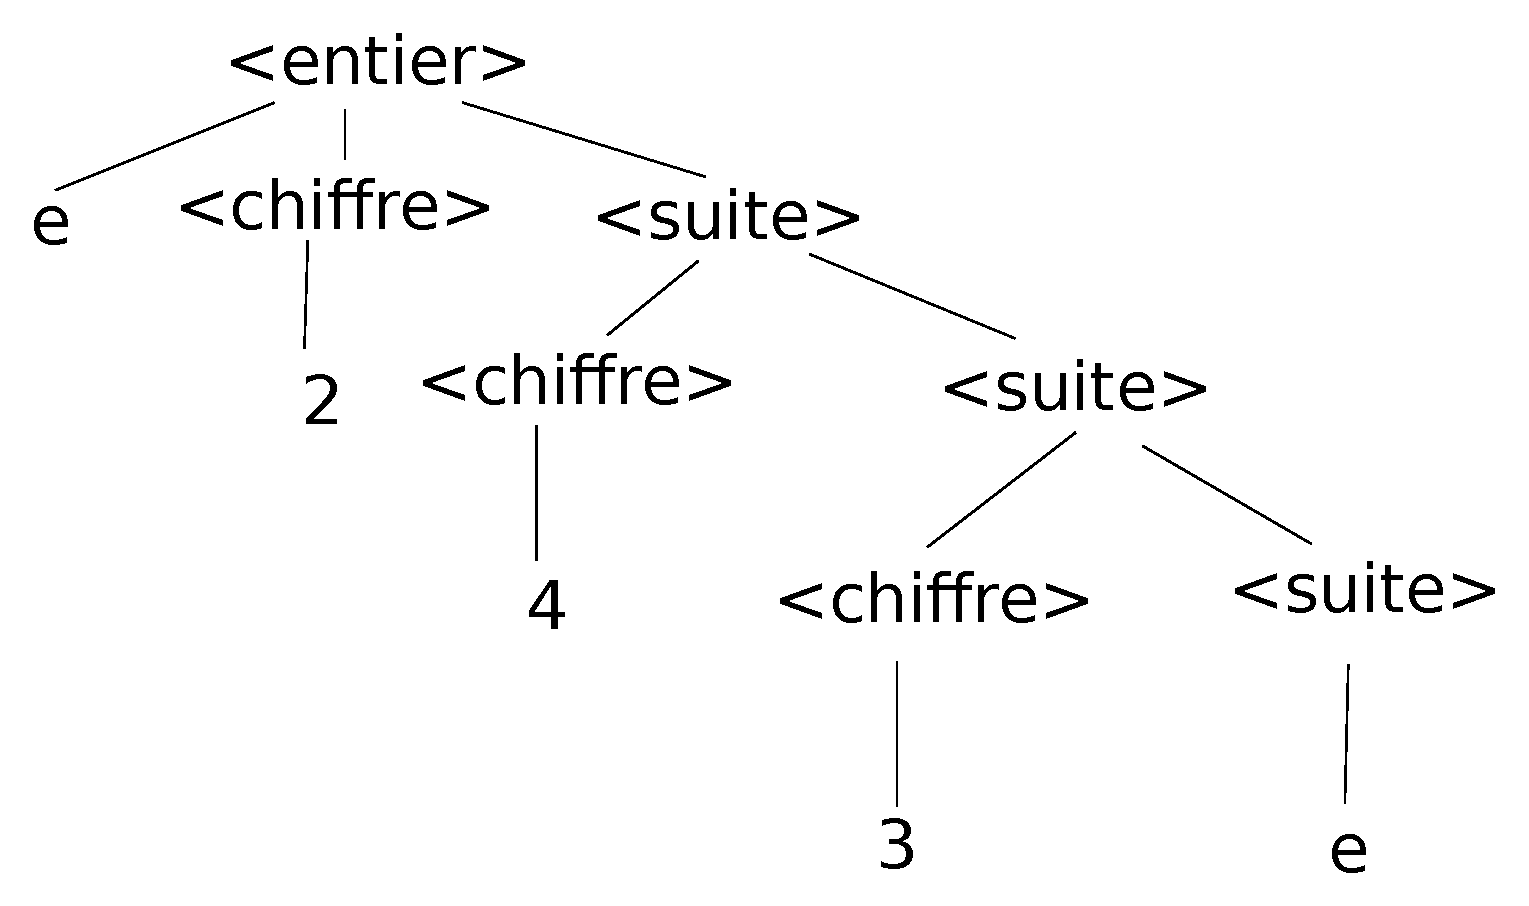
\includegraphics[width=\linewidth]{fig1_graphe_BNF_entier.pdf}




\fiche{Notion d'algorithme}
\titre{Théorie de la calculabilité} : Cactérisation des fonctions calculables sous forme d'un algorithme.\\

\titre{Exemple} : Savoir à partir d'un couple (algorithme, données initiales) si l'algorithme se termine ou pas n'est pas calculable. \\

\titre{Preuve} : L'ensemble des algorithmes est dénombrable (car un algorithme est un mot fini sur un alphabet fini), tandis que les fonctions ne sont pas dénombrable (théorème de Cantor). \\

\titre{Théorème de Cantor} : Il n'existe pas de bijection entre $E$ et $P(E)$.\\

\titre{Preuve} : \begin{enumerate}
	\item Il existe une injection triviale de $E$ dans $P(E)$
	\item Supposons qu'il existe une bijection $f$ de $E$ dans $P(E)$ et considérons $D=\{x\in E \tq x\not\in P(E)\}$. \\
Comme $f$ est bijective, $\exist y\in E\tq f(y)=D$ \\
Si $y\in D$ alors $y\not\in f(y) = D$, Si $y\not\in D=f(y)$ alors $y\in D$\\
Contradiction
\end{enumerate}


\fiche{Complexité}
\titre{Deux calculs possibles} : \begin{itemize}
	\item Complexité en temps
	\item Complexité en espace (obsolète)
\end{itemize}

\titre{Méthode} : \begin{itemize}
	\item On choisit des \titre{opérations de référence} (celles qu'on va comptabiliser). Si on les choisit toutes, on dit qu'on réalise une \titre{analyse fine}.
	\item On calcule le nombre d'opérations de référence -> fonction de $n$ (nombre de données à l'entrée)
	\item On donne un \titre{ordre de grandeur asymptotique} en $O(f(n))$ où $f \in \{ \ln(n),n,n^2 \}$
\end{itemize}



\fiche{Arbres Binaires}
\titre{Arbre binaire} : Structure de donnée soit $\vide$ soit $<o,A_g,A_d>$ avec : 
\begin{itemize}
	\item $o$ est un élément (noeud) de l'arbre appelé \titre{racine}
	\item $A_g$ et $A_d$ sont des arbres binaires disjoints appelés sous arbre gauche et sous arbre droit.
\end{itemize} 

\titre{Arbre étiqueté} : On crée une fonction de l'ensemble des noeuds dans un ensemble $A$ donné. \\

\titre{Vocabulaire} :
	\titre{Fils droit}
	,\titre{Fils gauche}
	,\titre{Point simple}
	,\titre{Point double}
	,\titre{Noeaud interne}
	,\titre{Feuille}
\\

\titre{Cas particuliers} \begin{itemize}
	\item \titre{Arbre parfait}
	\item \titre{Arbre complet}
	\item \titre{Arbre dégénéré ou filiforme}
	\item \titre{Localement complet} (pas de point simple)
	\item \titre{Arbre trié}
\end{itemize}




\fiche{Parcours d'un arbre}
\begin{center}

\titre{Ordre préfixe} (pré-ordre) :\\
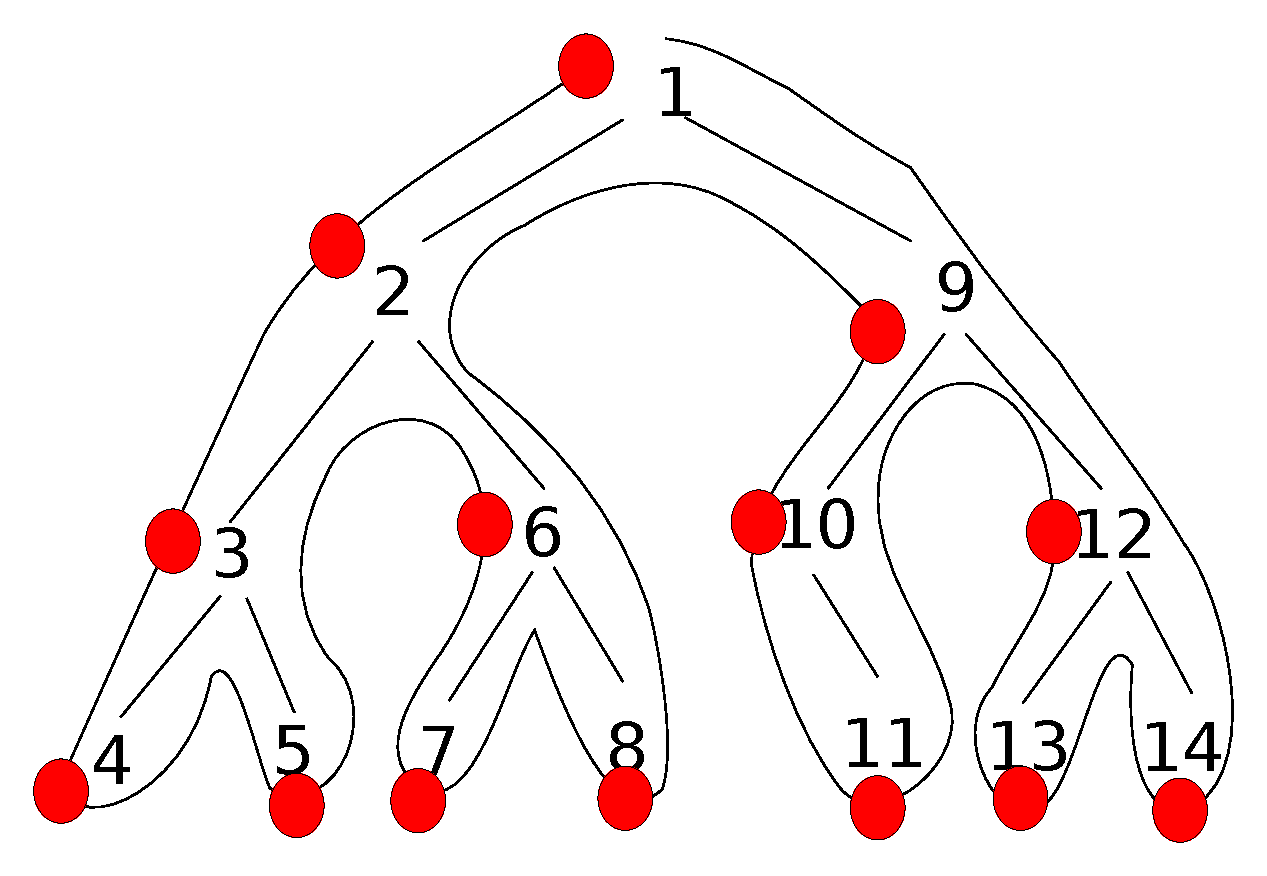
\includegraphics[width=0.5\linewidth]{fig2_prefixe.pdf}

\titre{Ordre infixe} :\\
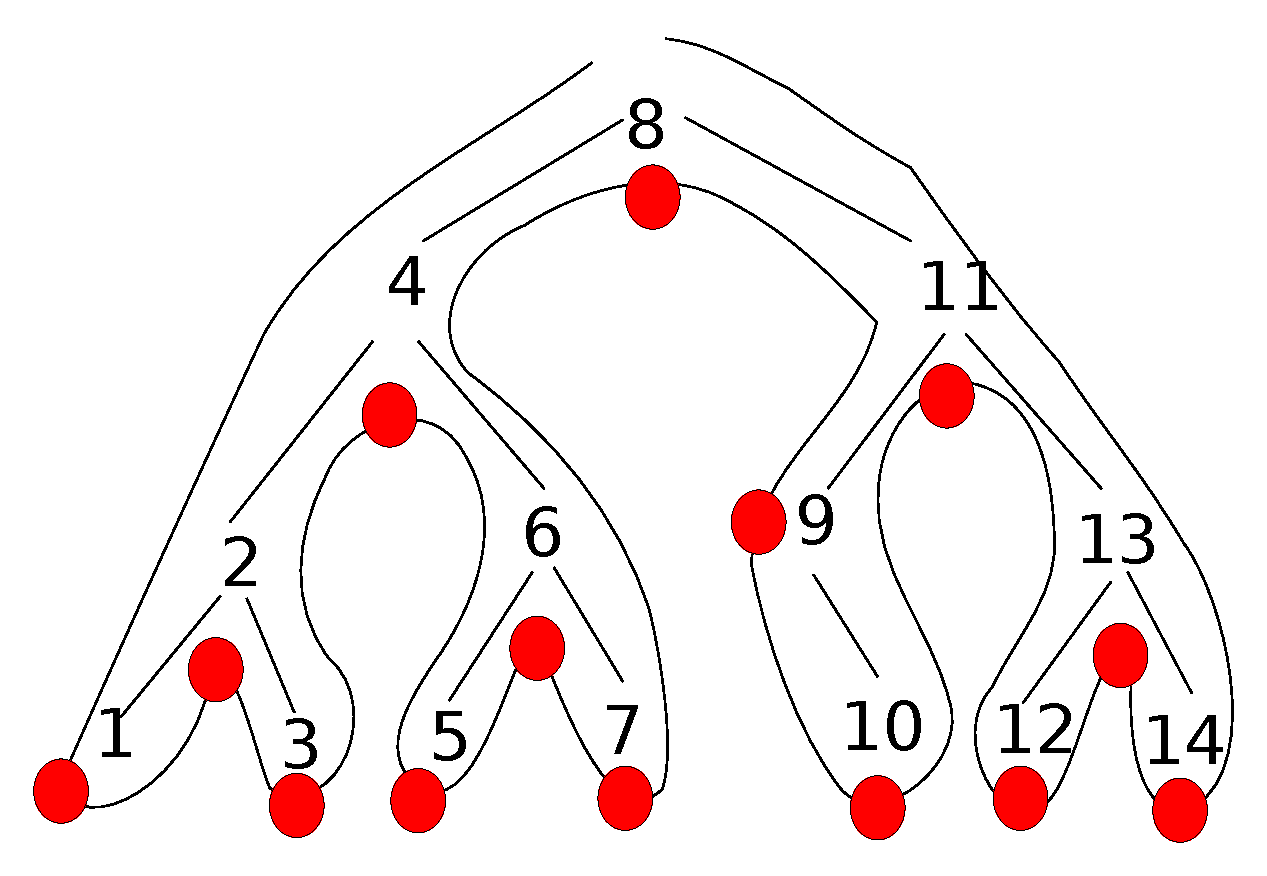
\includegraphics[width=0.5\linewidth]{fig3_infixe.pdf}

\titre{Ordre suffixe} :\\
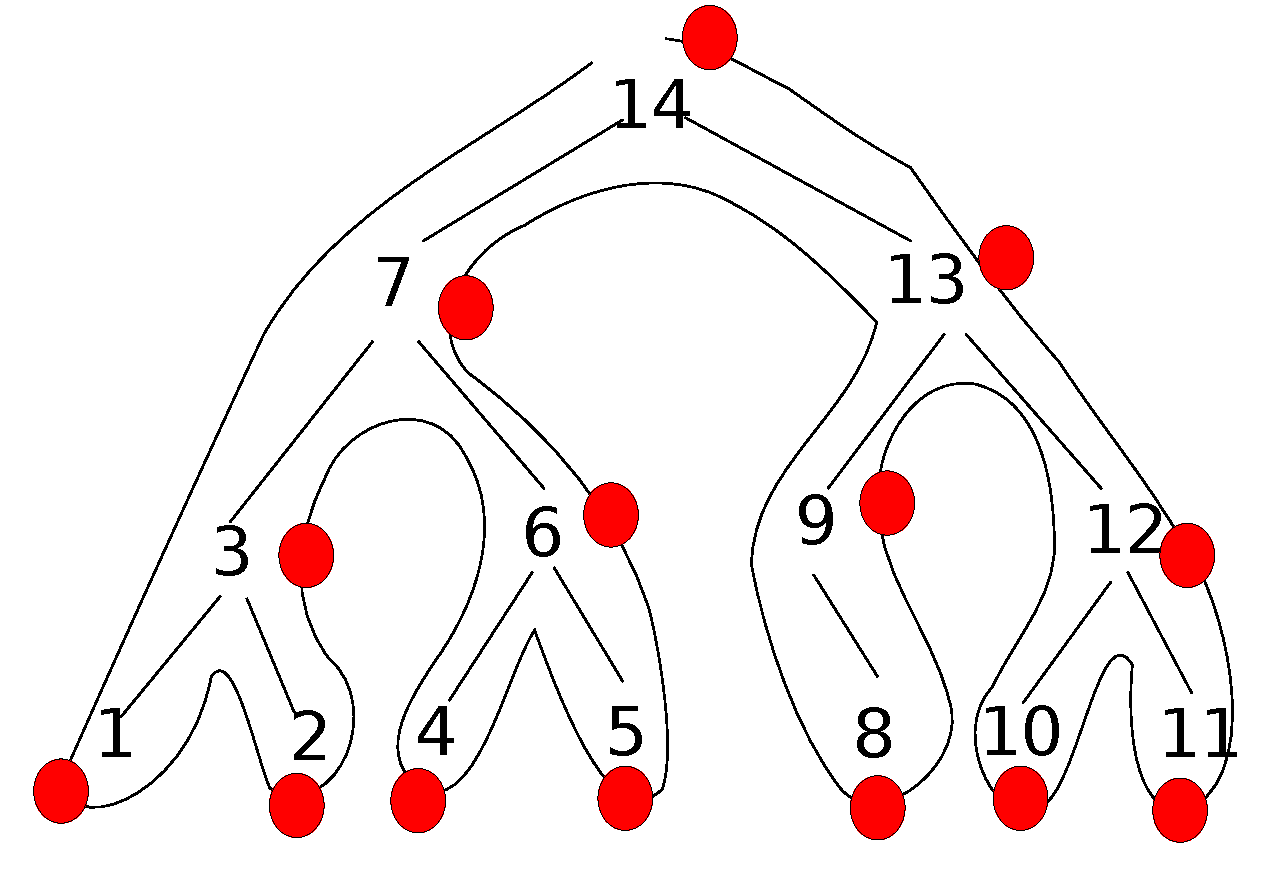
\includegraphics[width=0.5\linewidth]{fig4_suffixe.pdf}

\end{center}


\fiche{Rotations}
\begin{center}

\titre{Rotations simples} :\\
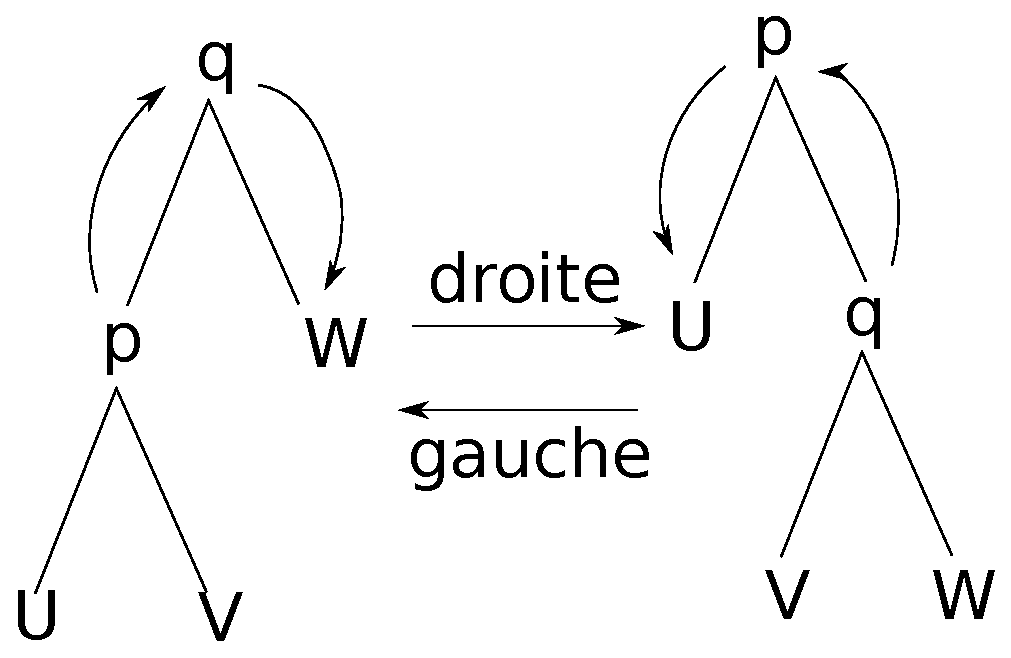
\includegraphics[width=0.5\linewidth]{fig5_rotations_simples.pdf}\vskip 0.2cm

\titre{Rotation droite-gauche} :\\
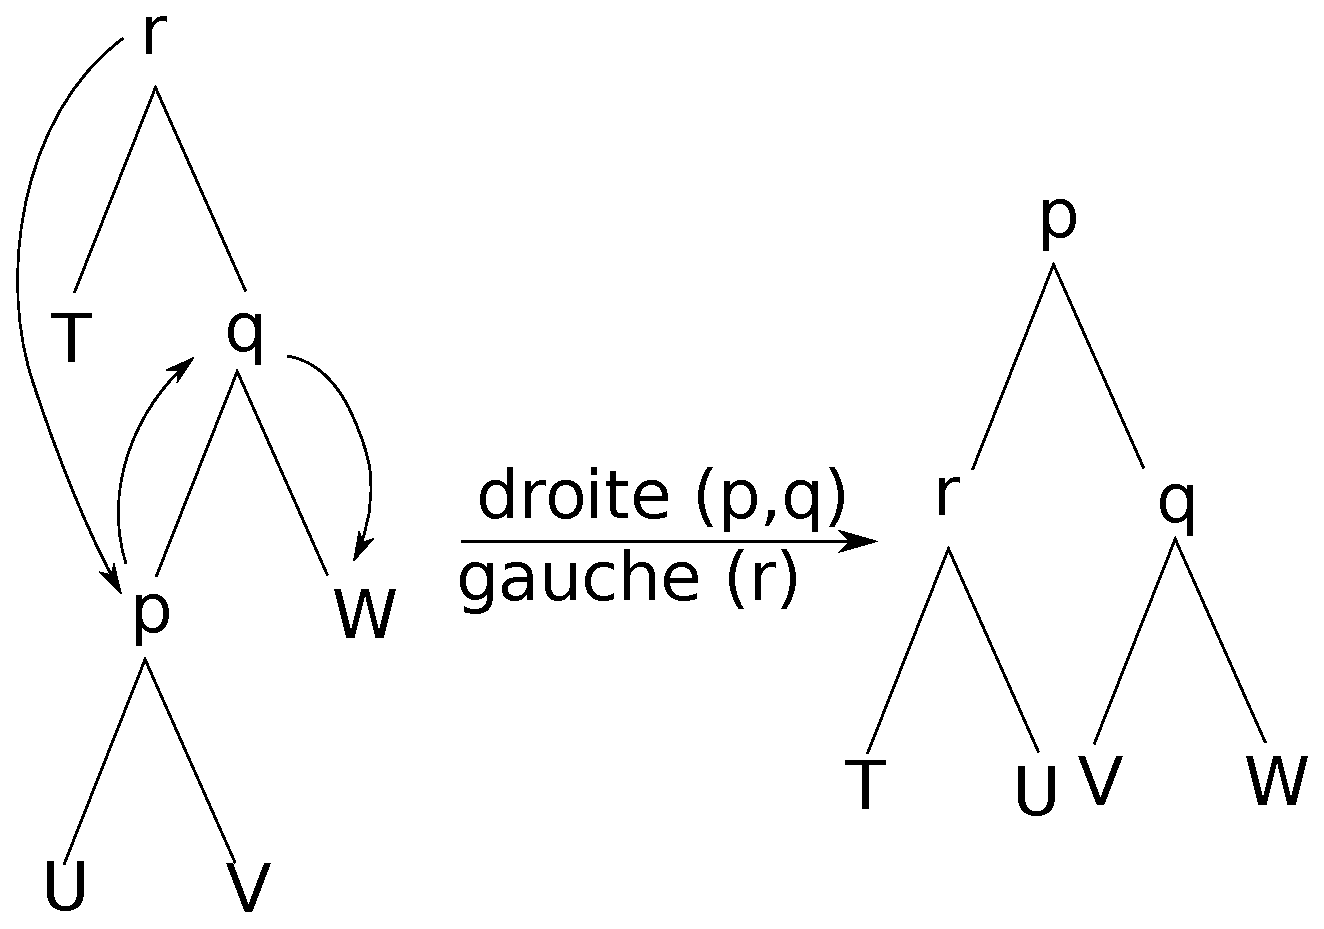
\includegraphics[width=0.5\linewidth]{fig5_rotation_dg.pdf}\vskip 0.2cm

\titre{Rotation gauche-droite} :\\
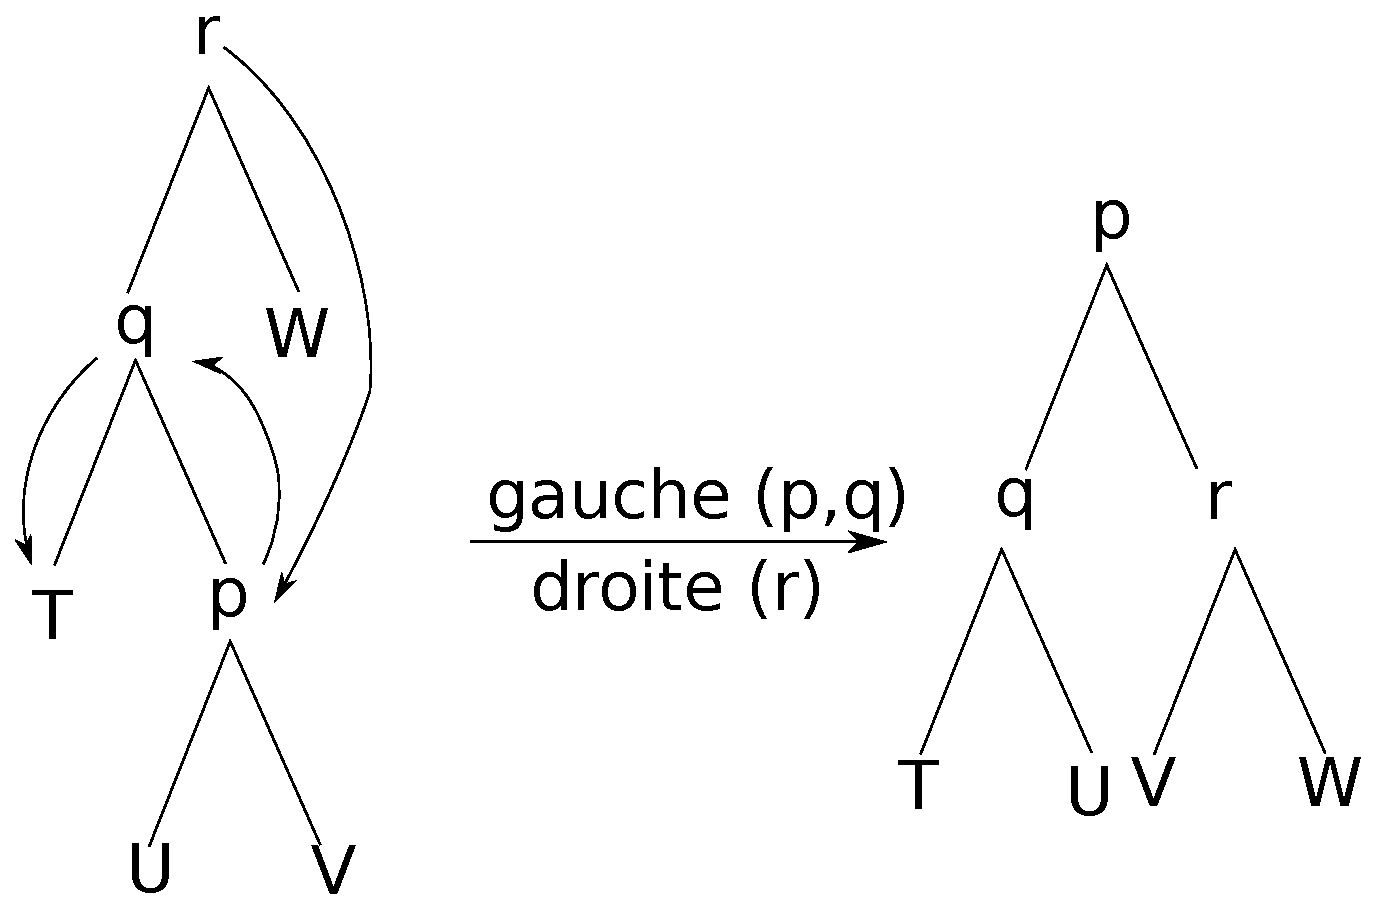
\includegraphics[width=0.5\linewidth]{fig5_rotation_gd.pdf}\vskip 0.2cm

\end{center}


\fiche{AVL}
\titre{Arbre AVL} : C'est un arbre trié dans lequel en tout noeud les hauteurs du sous arbre droit et du sous arbre gauche diffèrent d'au plus 1. \\

\titre{Construction de l'arbre} : On place les éléments dans l'arbre trié. 
\begin{enumerate}
  \item Si on crée un déséquilibre à l'extrême gauche on fait une rotation droite.
  \item Si on crée un déséquilibre dans la partie gauche on fait une rotation gauche-droite.
  \item Si on crée un déséquilibre à l'extrême droite on fait une rotation gauche.
  \item Si on crée un déséquilibre dans la partie droite on fait une rotation droite-gauche. 
\end{enumerate}

\titre{Choix du noeud} : On fait la rotation sur le noeud le plus bas parmis les noeuds en déséquilibre.\\

\titre{Suppression d'un élément} On part du père de l'élément supprimé et on remonte jusqu'à la racine en faisant des rotations à chaque fois qu'on a un déséquilibre.



\fiche{Exemple}
\titre{Exemple} : $\{18,98,51,70,62,13,29,33,57,61,35,15,3\}$ \\

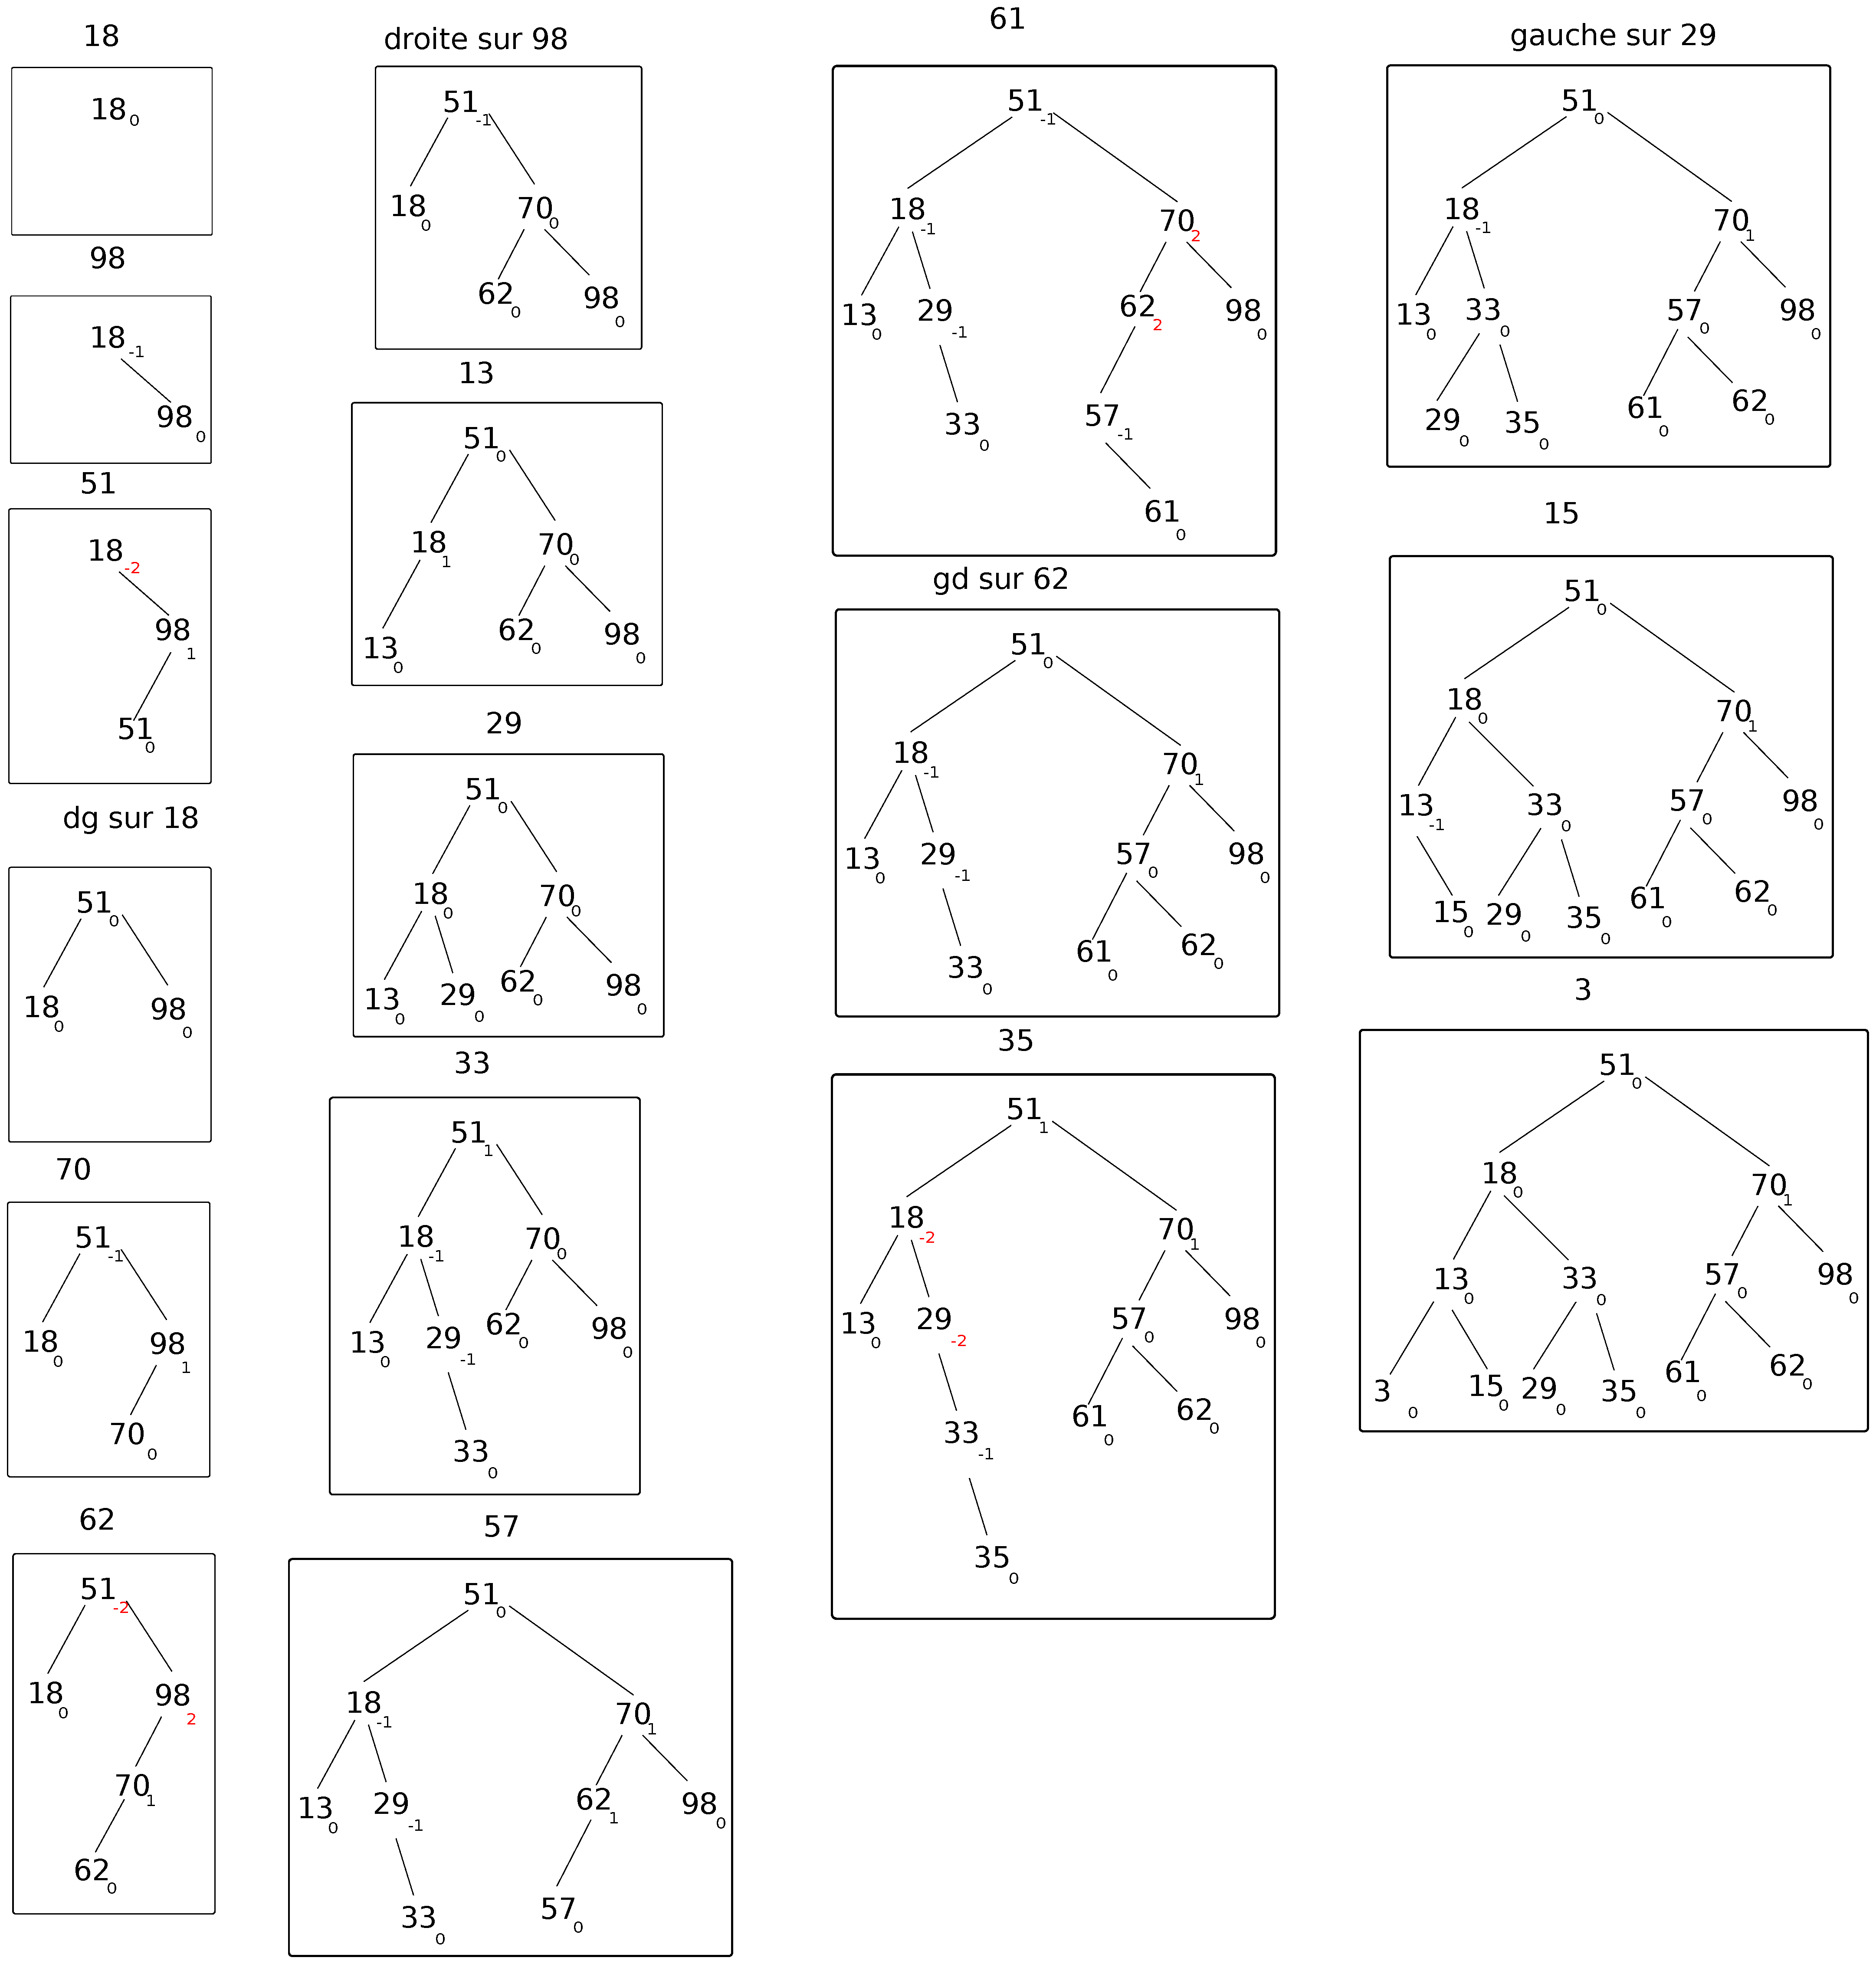
\includegraphics[width=\linewidth]{fig6_exemple.pdf}

\end{document}
